\documentclass[11pt,a4paper]{ivoa}
\input tthdefs

\usepackage{tikz}
\usetikzlibrary{positioning}

\lstloadlanguages{XML}
\lstset{flexiblecolumns=true,tagstyle=\ttfamily,
showstringspaces=False,basicstyle=\footnotesize}

\definecolor{termcolor}{rgb}{0.6,0.1,0.1}
\iftth
\def\vocterm#1{\emph{\color{termcolor}#1}}

\else
\def\vocterm{\startvocterm\realvocterm}
\def\realvocterm#1{\emph{\color{termcolor}#1}\endvocterm}
\begingroup
\gdef\breakablecolon{:\hskip0pt}
\catcode`\:=\active
\gdef\startvocterm{\begingroup
  \catcode`\:=\active\let:=\breakablecolon}
\gdef\endvocterm{\endgroup}
\endgroup
\fi

\title{TableReg: Registering TAP-Queriable Tables Conforming to Standard
Schemas}

% see ivoatexDoc for what group names to use here; use \ivoagroup[IG] for
% interest groups.
\ivoagroup{Registry}

\author[http://www.ivoa.net/cgi-bin/twiki/bin/view/IVOA/MarkusDemleitner]{Markus Demleitner}

\editor{Markus Demleitner}

\previousversion{This is the first public release}


\begin{document}
\begin{abstract}
An increasingly popular pattern in the Virtual Observatory, pioneered
by Obscore, is to define a schema for one or more tables in a database
and then publish data by making it accessible in tables conforming to
that schema in TAP services.  This document discusses how such resources
should be represented in the VO Registry to facilitate data discovery,
in particular global, all-VO data discovery.

It turns out that the existing registration patterns for Obscore,
RegTAP, and EPN-TAP require some adjustments.  The document therefore
also proposes transition strategies for these.
\end{abstract}


\section*{Conformance-related definitions}

The words ``MUST'', ``SHALL'', ``SHOULD'', ``MAY'', ``RECOMMENDED'', and
``OPTIONAL'' (in upper or lower case) used in this document are to be
interpreted as described in IETF standard RFC2119 \citep{std:RFC2119}.

The \emph{Virtual Observatory (VO)} is a
general term for a collection of federated resources that can be used
to conduct astronomical research, education, and outreach.
The \href{https://www.ivoa.net}{International
Virtual Observatory Alliance (IVOA)} is a global
collaboration of separately funded projects to develop standards and
infrastructure that enable VO applications.


\section{Introduction}

Beginning with Obscore 1.0 \citep{2011ivoa.spec.1028T}, an increasing
number of Virtual Observatory standards at their core just define a
table schema -- understood here as a well-defined set of columns within
one or more relations -- and rely on TAP \citep{2019ivoa.spec.0927D} to
let clients actually run queries.  Standards of this type include:

\begin{itemize}
\item Obscore \citep{2017ivoa.spec.0509L} -- a table for metadata of
observational data products
\item RegTAP \citep{2019ivoa.spec.1011D} -- a 13-table schema with
metadata of VO resources
\item ObsLocTAP \citep{2021ivoa.spec.0724S} -- a table schema to
communicate plans for observations and metadata of completed
observations
\item EPN-TAP \citep{2022ivoa.spec.0822E} -- a table schema for solar
system data
\end{itemize}

More such standards are currently being developed. Examples include LineTAP
\citep{wd:linetap23} and the Obscore extension for radio data.

Of course, resources complying to these standards must be made
discoverable to be useful.  Both Obscore and RegTAP have employed the
\xmlel{dataModel} element specifically introduced into TAPRegExt
\citep{2012ivoa.spec.0827D} to declare the presence of tables adhering
to a standard schema in a TAP service.

Both Obscore and RegTAP are singletons with fixed names, i.e., once one
has discovered a TAP service ``supporting'' a data model, it is clear
how to query it.  However, even for these, the \xmlel{dataModel}-scheme
has severe shortcomings:

\begin{enumerate}
\item Lack of resource metadata: In resource records located during
discovery, the global VOResource metadata (title, authors, and perhaps
most importantly coverage in space, time and spectrum) are these of the
TAP service, which the tables may share with any number of other tables.

\item Unclear relationships: In particular for Obscore -- rather
typically serving several data collections at once --, a serious
problem is that data collection records can only generically say
that they are served by the TAP service (cf.~\citet{2019ivoa.spec.0520D}
for the general scheme of relating data collections and services).  From
that, clients cannot deduce whether the data is available through, say,
obscore, or only in some custom table.

\item Suitability: Adherence to a data model simply is not a property of a
TAP service.  It is a property of a specific table or schema.
\end{enumerate}

EPN-TAP then employed the table-in-TAP scheme without the constraint to
a singleton; since each data collection has an EPN-TAP table of its own,
the discovery process somehow also had to yield a table name.  As a
solution, the standard forsees using the table's \xmlel{utype} field in
the VODataService \citep{2010ivoa.spec.1202P} \xmlel{tableset}.

This mode of discovery was subsequently also employed in ObsLocTAP and
LineTAP.  It still has a drawback, though: Clients discovering a service
with a \xmlel{table} (or \xmlel{schema} in the case of RegTAP) with the
bespoke \xmlel{utype} have a hard time determining whether what they
have found is the data collection's record (and hence the global
metadata pertains to the data collection itself) or the record of the
TAP service serving the data collection (in which case the global
metadata pertains to the TAP service and will be essentially unrelated
to the data collection in question).

This note remedies that by prescribing that for resource records for
standard-compliant tables, the resource type \xmlel{vs:CatalogResource}
must be used.

In Sect.~\ref{sect:norms}, we review the proposed scheme and give
boilerplate text to include in standards following it.  One reason to
introduce the scheme is to enable expressing inclusion relationships
between resources for the benefit of clients doing global discovery.
Sect.~\ref{sect:rels} discusses this mechanism in more detail.  Finally,
Sect.~\ref{sect:transition} addresses the question of how to transition
from what the standards currently say (and the services and clients
implement) to a VO adopting the scheme proposed here.

\section{Registering and Discovering Standard Tables}
\label{sect:norms}

In the scheme proposed here, TAP-queriable resources conforming to
standard table schemas will be registered as
\xmlel{vs:CatalogResource}-typed Resources.  If they consist of only a
single table or of multiple, independently publishable tables (e.g.,
Obscore, EPN-TAP), an IVOA identifier \citep{2016ivoa.spec.0523D} is
defined for this particular table type.  This will refer to a StandardsRegExt
\citep{2012ivoa.spec.0508H} \xmlel{StandardKey}, generally in the
defining standard's resource record.  This standard key SHOULD contain a
version tag precise to the minor version; it is at least conceivable
that clients may only want to discover tables containing later
additions.

Hence, the VODataService \xmlel{table} element for a table conforming to
Obscore 1.2 would begin like this:
\begin{lstlisting}[language=XML]
<table>
  <name>ivoa.obscore</name>
  <title>Obscore Table in the Fictional Data Centre</title>
  <description>
    This is example metadata for use in the
    TableReg specification.
  </description>
  <utype>ivo://ivoa.net/std/obscore#table-1.2</utype>
  ...
\end{lstlisting}
where Obscore's StandardsRegExt record contains a fragment:
\begin{lstlisting}[language=XML]
<key>
  <name>table-1.2</name>
  <description>The data model for a table conforming to version 1.2
  of this specification.  This implies a set of nn mandatory columns,
  as well as the table's name, ivoa.obscore.
  </description>
</key>
\end{lstlisting}

Standards defining full schemas, i.e., sets of interconnected tables
that only make sense together -- at the moment, RegTAP is our only
example -- will similarly define a StandardKey to use with a schema
element.  The RegTAP registry record currently has:

\begin{lstlisting}[language=XML]
<key>
  <name>1.1</name>
  <description>The data model for the tables making up the relational
  registriy in version 1.1.  This key is used to locate TAP services
  implementing RR in TAPRegExt dataModel or VODataService schema/@utype
  elements.
  </description>
</key>
\end{lstlisting}

Hence, the tableset of the record for the Heidelberg RegTAP service
\nolinkurl{ivo://org.gavo.dc/rr/q/create} contains:

\begin{lstlisting}[language=XML]
<schema>
   <name>rr</name>
   <title>GAVO RegTAP Service</title>
   <description>
     Tables containing the information in the IVOA Registry[...]
   <utype>ivo://ivoa.net/std/RegTAP#1.1</utype>
   <table>...
\end{lstlisting}

It is not recommended to follow the RegTAP's example of omitting an
indicator of what is referred to in the standard key's name.  Hence,
prefer, for instance, \verb|schema-1.1| to \verb|1.1|; it is always
conceivable that additional versioned entities may require standard
keys.

Let us stress that for standard discovery, the minor
version must be ignored.  Clients should be written such that if they
work for any 1.x version, they work for all 1.x versions, except of
course where compelling reasons exist to require features not present in
earlier minor versions.


\section{Expressing Relationships Between Tables and Other Resources}
\label{sect:rels}

An important reason to enumerate resources conforming to a schema is
global discovery of whatever is described in the table; in the case of
Obscore, this would be observational datasets.

\begin{figure}
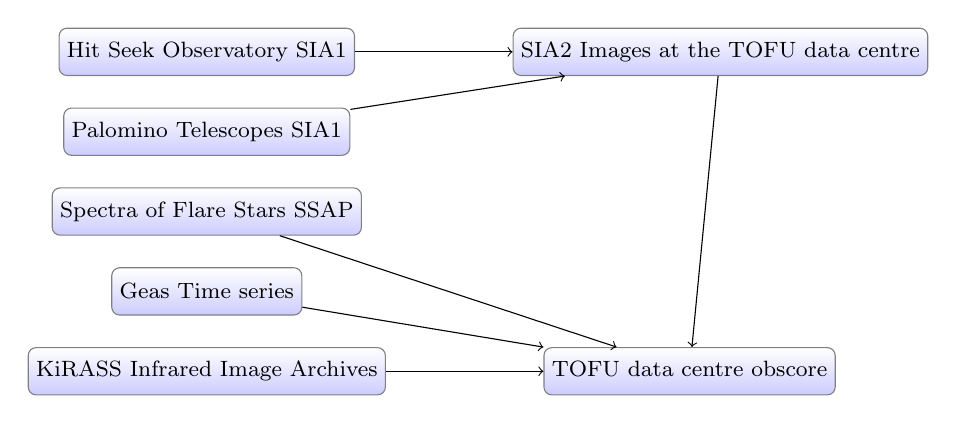
\begin{tikzpicture}[
service/.style={bottom color=blue!20,
  top color=white,
  rounded corners=1mm,
  minimum height=6mm,
  thin,draw=black!50,align=center,
  node distance=4mm and 2cm,
  node font=\footnotesize
}]
\node (s1) [service] {Hit Seek Observatory SIA1};

\node (s2) [service, below=of s1] {Palomino Telescopes SIA1} ;

\node (s3) [service, below=of s2] {Spectra of Flare Stars SSAP} ;

\node (s4) [service, below=of s3] {Geas Time series};

\node (s5) [service, below=of s4] {KiRASS Infrared Image Archives};

\node (s6) [service, right=of s1] {SIA2 Images at the TOFU data centre};

\node (s7) [service, right=of s5] {\strut TOFU data centre obscore};


\draw [black,->] (s1) to (s6);
\draw [black,->] (s2) to (s6);
\draw [black,->] (s3) to (s7);
\draw [black,->] (s4) to (s7);
\draw [black,->] (s5) to (s7);
\draw [black,->] (s6) to (s7);
\end{tikzpicture}

\caption{Benefits of making relationships between resources explicit.
The nodes in this graph correspond to services, the arrows point from a
a service to a collective service also serving the data served by the
first service.  By evaluating the relationships, a
client can deduce that the data published through the seven services
can be queried by running one Obscore query on the TOFU data
centre.}
\label{fig:rel-sketch}
\end{figure}

Furthermore, an important reason to define
registry records for such resources is
that data collections published using multiple standards or through
multiple services can
machine-readably declare that querying one such resource is enough to
cover the entire data available.  In that way, clients
doing global discovery can skip services publishing data they already
queried using other services.  Consider Fig.~\ref{fig:rel-sketch} for an
illustration of the dramatic savings enabled by making such
relationships explicit.

In VOResource, relationships are declared between registry resources
using the \xmlel{relationship} element, containing a
\xmlel{relationshipType} and one or more \xmlel{relatedResource}-s.  For
relationships between data collections and services making them
queriable, the Endorsed Note on Discovering Data Collections
\citep{2019ivoa.spec.0520D} prescribes \vocterm{IsServedBy} from the IVOA
relationship type
vocabulary\footnote{\url{http://www.ivoa.net/rdf/voresoure/relationship_type}}.

We argue that this term can be re-used here, even though the
relationship's label might appear somewhat misplaced when a
CatalogService-typed record declares that it is served by a
CatalogResource-typed record; that is what happens if a SIA-published
data collection says it is also present in an obscore table.

More specifically, where data contained in or published through resource
$A$ is also contained in or published through a more general (in the sense
of: making other data collections queriable, too) resource $B$, the
resource record of record $A$ should declare a relationship to $B$ with
a \xmlel{relationshipType} of \vocterm{IsServedBy}.

Resources MUST NOT declare circular \vocterm{IsServedBy} relationships.

\section{Transitioning to a TableReg World}
\label{sect:transition}


\section{Obscore Tables in the Registry}

This section is intended both as the blueprint for what Obscore 1.2
should say (in addition to the transitional \xmlel{dataModel}
declaration in the capabilities) and as a template on which to base
the Registry sections of similar standards.

\subsection{Registering Obscore Tables}
\label{sect:registering-obscore}

Obscore tables are registered using VODataService
\citep{2010ivoa.spec.1202P} tablesets, where the table utype is set to
$$\hbox{\verb|ivo://ivoa.net/std/linetap#table-1.0|}.$$

The tableset is contained in a VODataService \xmlel{vs:CatalogResource}
record with a TAP capability, where this capability is an auxiliary
capability as per DDC \citep{2019ivoa.spec.0520D}.  The TAP service
serving the table must also be registered, and an \vocterm{IsServedBy}
relationship must be declared from the Obscore record to the TAP record.

When registry records for data collections published through the Obscore
table are also published -- and publishers are strongly urged to do
that whenever the Obscore record does not contain the Dublin Core
metadata for the individual collection(s) --, \vocterm{IsServedBy}
relationship must also be declared from the individual collections'
records to the Obscore record.

An example for a registry record in VOResource, for the case of
using an auxiliary capability referencing a main TAP service comes with
this document\footnote{\auxiliaryurl{example-record.xml}}.

The noteworthy points in the record are:

\begin{itemize}
\item A \xmlel{relationship} element referencing the main TAP service
through which the service is queriable as per DDC:
\begin{lstlisting}[language=XML,basicstyle=\footnotesize]
<relationship>
  <relationshipType>IsServedBy</relationshipType>
  <relatedResource ivo-id="ivo://org.gavo.dc/tap"
    >GAVO Data Center TAP service</relatedResource>
</relationship>
\end{lstlisting}

\item The declaration for the auxiliary capability, including the access
URL so clients do not need to follow the relationship just declared if
all they need is the access URL:
\begin{lstlisting}[language=XML,basicstyle=\footnotesize]
<capability standardID="ivo://ivoa.net/std/TAP#aux">
   <interface role="std" version="1.1" xsi:type="vs:ParamHTTP">
     <accessURL use="base">http://dc.zah.uni-heidelberg.de/tap</accessURL>
   </interface>
</capability>
\end{lstlisting}

\item Most importantly, the declaration of the table utype that lets
clients discover that this particular table contains Obscore data:
\begin{lstlisting}[language=XML,basicstyle=\footnotesize]
<table>
  <name>ivoa.obscore</name>
  <title>GAVO Data Center Obscore Table</title>
  <description>The IVOA-defined obscore table, containing generic
  metadata for datasets within this datacenter.</description>
  <utype>ivo://ivoa.net/std/obscore#table-1.1</utype>
  ...
</table>
\end{lstlisting}
\end{itemize}

\subsection{Discovering Obscore Tables}

Obscore clients in general are interested in TAP endpoints of Obscore
services as well as the table's metadata, such as its coverage in space,
time, and spectrum.  By the  registration pattern given in
\ref{sect:registering-obscore}, this translates into resources with TAP
(auxiliary) capabilities that have a standard key for version 1 Obscore
in a table utype; this will normally also match the TAP service record
itself (as it generally also gives the tableset). Therefore, an
additional constraint on the record type is introduced.

Translated into RegTAP \citep{2019ivoa.spec.1011D}, the following query
would return TAP access URLs and the table names:

\begin{lstlisting}[language=SQL]
SELECT DISTINCT table_name, access_url
FROM rr.res_table
  NATURAL JOIN rr.capability
  NATURAL JOIN rr.interface
WHERE
  table_utype LIKE 'ivo://ivoa.net/std/obscore#table-1.%'
  AND standard_id LIKE 'ivo://ivoa.net/std/tap%'
  AND intf_role='std'
  AND res_type='vs:catalogresource'
\end{lstlisting}

The regular expression in the utype match is to make sure minor version
increments do not prevent resource discovery; by IVOA versioning rules,
all LineTAP services of minor version 1 can be operated by all LineTAP
clients of version 1.  We do not constrain the version of the TAP
service. Clients may want to adapt the TAP discovery pattern to match
their specific needs.

Clients can add additional constraints (e.g., on publishers, coverage,
or, in VODataService 1.3 or later, data product types) to this basic
query as usual in VOResource (i.e., by \verb|NATURAL JOIN|-ing the
tables containing the columns and adding additional \verb|WHERE|
clauses.  Constraints against the embedding TAP service, however,
require a more complex join through the \verb|rr.relationship| table;
this is not expected to be a common use case.

For Obscore 1.3, \verb|table_name| in this query will always be
\verb|ivoa.obscore|.  This item hence is only relevant for standards
that allow for flexible table names.

\appendix
\section{Changes from Previous Versions}

No previous versions yet.
% these would be subsections "Changes from v. WD-..."
% Use itemize environments.


% NOTE: IVOA recommendations must be cited from docrepo rather than ivoabib
% (REC entries there are for legacy documents only)
\bibliography{ivoatex/ivoabib,ivoatex/docrepo,local}


\end{document}
